\section{System architecture and cross-event recovery framework}
\label{sec:system}

\subsection{Physical architecture of the system}
\label{sec:architecture}

The AI data center integrated energy system (AIDC-IES) considered in this paper is shown in \figref{fig:arch}. It
hosts $N=16{,}000$ H100-class GPUs in 2,000 eight-GPU nodes and is supplied by the utility grid through a connection
limited to $\Pcap=\gamma\hat P$, where $\hat P$ is the peak import on a typical day and $\gamma$ is the connection
margin. On site, an 8-MWp photovoltaic (PV) array, a 3-MW gas engine whose waste heat drives an absorption chiller,
temperature-dependent electric chillers, a 10-MWh chilled-water thermal energy storage (TES) and a 6-MW/12-MWh battery
energy storage system (BESS) form an electricity--cooling--heat coupled energy system. The information layer consists of
the grid operator or aggregator, which issues DR events under the Jiangsu rules~\cite{jiangsu2024dr}, the day-ahead
commitment, the intraday rolling joint-recovery controller and the execution and settlement layer.

\begin{figure*}[!t]
\centering
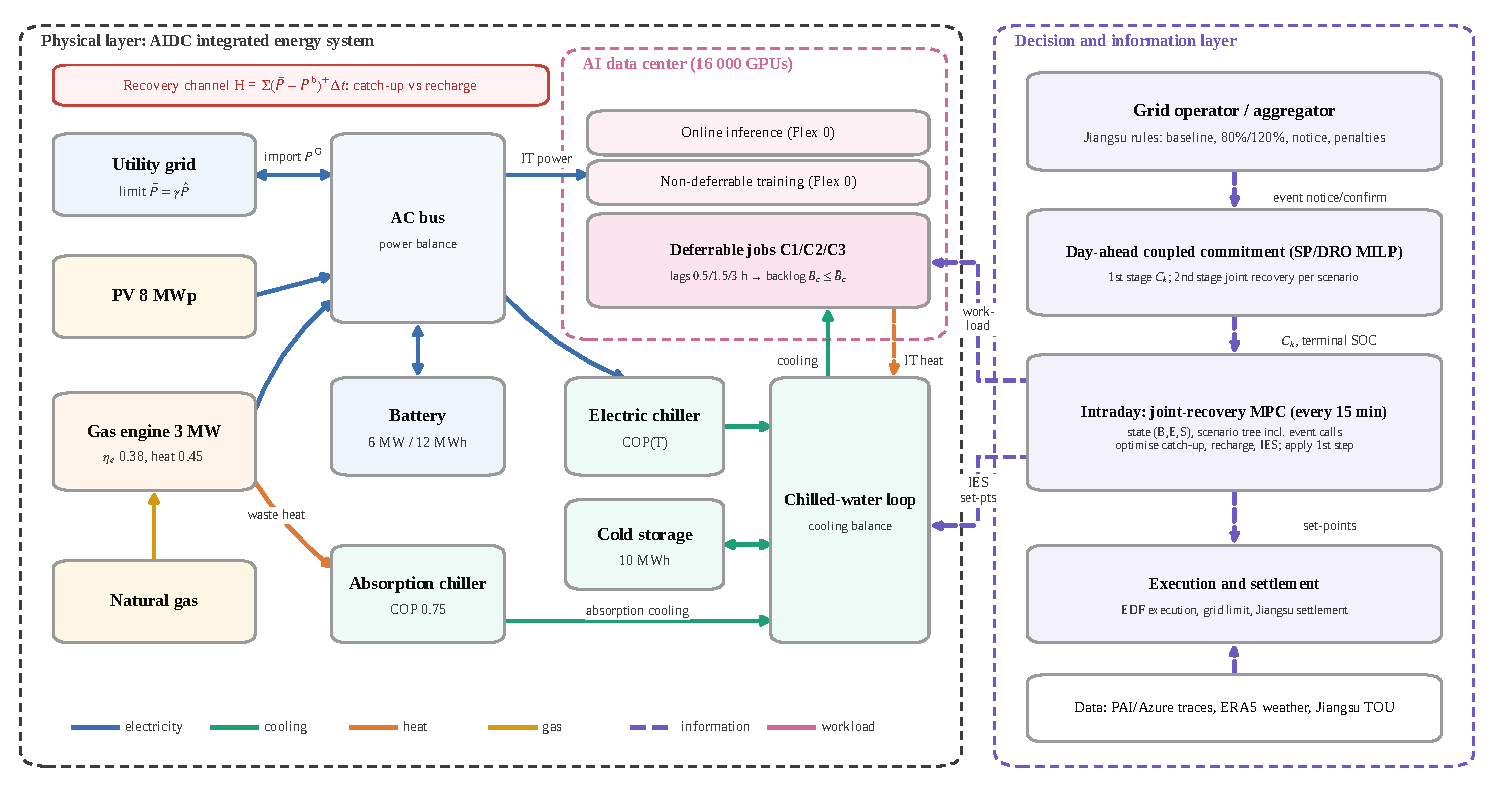
\includegraphics[width=0.98\textwidth]{fig00_architecture.pdf}
\caption{Physical and information architecture of the AI data center integrated energy system (AIDC-IES). The
recovery channel is the connection headroom above the DR baseline that is shared by catch-up computing and storage
recharging between events.}
\label{fig:arch}
\end{figure*}

The GPU workload is divided into tiers that follow the flexibility levels used in AI data center DR
programs~\cite{colangelo2025} (\tabref{tab:tiers}). Online inference, whose shape follows the Azure LLM inference
trace~\cite{stojkovic2025}, and the non-deferrable part of training are served immediately. Deferrable training and
batch jobs from the Alibaba PAI GPU trace~\cite{weng2022} are split by run time into short, medium and long classes
with lag bounds $L_c$ of 0.5, 1.5 and 3~h, \ie\ every unit of work must be completed within $L_c$ of its nominal
completion time.

\begin{table}[!t]
\caption{Workload tiers of the AI data center.}
\label{tab:tiers}
\centering\footnotesize
\begin{tabular}{@{}llll@{}}
\toprule
Tier & Source & Deferrable & Lag bound $L_c$\\
\midrule
Online inference & Azure LLM 2024~\cite{stojkovic2025} & No (Flex 0) & 0\\
Non-deferrable training & PAI $\times$ 25\%~\cite{weng2022} & No (Flex 0) & 0\\
C1 short jobs ($\le$1 h) & PAI $\times$ 75\% & Flex 1 & 0.5 h\\
C2 medium jobs (1--12 h) & PAI $\times$ 75\% & Flex 2 & 1.5 h\\
C3 long training ($>$12 h) & PAI $\times$ 75\% & Flex 3 & 3 h\\
\bottomrule
\end{tabular}
\end{table}

\subsection{Consecutive DR events and the recovery channel}
\label{sec:channel}

Three events are called on the case day. E1 (17:00--18:00) and E2 (19:00--20:00) are day-ahead agreed responses paid
3~CNY/kWh; E3 (21:00--22:00) is a fast peak-avoidance response that is pre-announced the day before and confirmed 3~h
ahead (speed coefficient 1.4, 4.2~CNY/kWh). In the uncertain variant, E3 is only announced as a possible event that is
called with probability 0.6 and confirmed or cancelled 1~h ahead (coefficient 1.6, 4.8~CNY/kWh).

Each event leaves a recovery state $\mathbf{x}_{e_k}=(B_1,B_2,B_3,E,S)$: the backlog of the three job classes and the
energy of the BESS and TES. The paper refers to the computing and storage sides as two kinds of recovery states; the
state vector has five dimensions, and one more each when data hall thermal inertia or a hot-water tank is modelled.
During the gap $\Iset_k$ between two events, catch-up computing and storage recharging draw on the same recovery
channel, whose energy is
\begin{equation}
H_k=\sum_{t\in\Iset_k}\big(\Pcap-\Pb_t\big)^+\dt ,
\label{eq:channel}
\end{equation}
minus the part that is charged as rebound in the post-event window. Catch-up computing and recharging compete for $H_k$
subject to the idle GPU capacity, the storage power limits and the job deadlines. Under independent recovery (IR) each
side recovers by its own rule or optimizer; under joint recovery (JR) the channel is allocated to the states that the
remaining events need most.

\subsection{Computing side: IT power and lag-bounded backlog}
\label{sec:computing}

With $\dt=0.25$~h and a window from 00:00 of day D to 06:00 of day D+1 (120 steps), the IT power follows the
idle-plus-dynamic model~\cite{fan2007}
\begin{equation}
\Pit_t=N\pidle+P^{\mathrm{oth}}+\pdyn\Big(\kappa^{\mathrm{inf}}G^{\mathrm{inf}}_t+G^{\mathrm{fix}}_t+\sum_{c}\big(y_{c,t}-\zeta_{c,t}\big)\Big),
\label{eq:pit}
\end{equation}
where $P^{\mathrm{oth}}=0.6$~MW is the storage and network IT power, $\kappa^{\mathrm{inf}}=0.65$ reflects that
inference GPUs seldom reach their thermal design power~\cite{patel2024}, and $\zeta_{c,t}$ is the dynamic power removed
by optional power capping (zero in the base case). The deferrable classes share the free GPU capacity,
\begin{equation}
\sum_c y_{c,t}\le u^{\max}N-G^{\mathrm{inf}}_t-G^{\mathrm{fix}}_t ,
\label{eq:gpucap}
\end{equation}
with $u^{\max}=0.95$, and their backlog evolves as
\begin{equation}
B_{c,t}=B_{c,t-1}+a_{c,t}-\big(y_{c,t}-w_{c,t}\big)\dt+o_c\,u_{c,t},
\label{eq:backlog}
\end{equation}
where $a_{c,t}$ is the nominal work arriving in step $t$, $w_{c,t}$ the throughput lost by capping and $o_c u_{c,t}$
the optional pause/resume overhead. The tiered SLA is imposed by the lag bound
\begin{equation}
B_{c,t}-v_{c,t}\le\Bbar_{c,t}:=\sum_{\tau=t-L_c/\dt+1}^{t}a_{c,\tau},\qquad v_{c,t}\ge0,
\label{eq:lag}
\end{equation}
where the overdue work $v_{c,t}$ is penalised at $\clate=1000$~CNY per GPU$\cdot$h and hour, which in effect makes
the deadlines hard constraints. The following lemma shows that \eqref{eq:lag} is exact.

\begin{lemma}[Exactness of the lag bound]\label{lem:edf}
For any execution sequence with $y_{c,t}\ge0$ and $B_{c,t}\ge0$ in the fluid model, the following statements are
equivalent: (i) the executed work can be assigned to arrival batches such that every unit of work meets its deadline;
(ii) under EDF execution every unit of work meets its deadline; (iii) $B_{c,t}\le\Bbar_{c,t}$ for all $t$.
\end{lemma}

The proof is given in \appref{app:proofs}. A constant queue limit $B_{c,t}\le\bar Q$, as used in virtual-queue
models~\cite{zhang2026bilevel}, allows overdue work in the backlog when $\bar Q>\Bbar_{c,t}$ (low arrivals) and forbids
feasible deferrals when $\bar Q<\Bbar_{c,t}$ (high arrivals). The bound $\Bbar_{c,t}$ is the time-varying capacity of a
virtual computing storage: the facility energy embodied in the backlog, $X_t=\varepsilon_t\sum_cB_{c,t}$ with
$\varepsilon_t=(1+a^{\mathrm{aux}}+\theta/\COP_t)\pdyn$, is ``discharged'' when work is deferred during an event and
``recharged'' by catch-up computing afterwards, with a round-trip efficiency close to one.

\paragraph{Optional computing-side features} Four extensions are used in the sensitivity and validation studies.
(i)~\emph{GPU power capping} during events: $\zeta_{c,t}\le r^{\max}y_{c,t}$ in event steps, and the throughput loss
is the perspective of a convex piecewise-linear power--throughput curve through the capping levels $(r_l,q_l)$,
\begin{equation}
w_{c,t}\ge s_l\,\zeta_{c,t}+i_l\,y_{c,t},\quad l=1,\dots,n,\qquad w_{c,t}\ge0,
\label{eq:capping}
\end{equation}
with slopes $s_l$ and intercepts $i_l$; one level $(0.30,0.12)$ gives $w=0.4\zeta$, \ie\ every unit of power reduction
leaves a recovery debt of 0.4 instead of 1 for pausing. (ii)~A \emph{rigid-job recovery bound} for gang-scheduled jobs,
which cannot run faster after a pause and only work off their delay after their nominal end,
\begin{equation}
y_{c,t}\le a_{c,t}/\dt+B_{c,t-1}/\tau_c ,
\label{eq:rigid}
\end{equation}
where $\tau_c$ is the gang-weighted mean run time of the class (0.26/3.6/26.3~h for PAI and 0.11/4.2/39.5~h for the
Acme LLM trace~\cite{hu2024acme}); without \eqref{eq:rigid} the model is the fluid model of the base case.
(iii)~\emph{Pause/resume overheads}: $u_{c,t}\ge(a_{c,t}/\dt-y_{c,t})-(a_{c,t-1}/\dt-y_{c,t-1})$, $u_{c,t}\ge0$, and
every newly paused GPU adds $o_c$ GPU$\cdot$h of checkpoint and restart work. (iv)~An \emph{IT ramp limit}
$|\sum_c(y_{c,t}-y_{c,t-1})|\pdyn\le R^{\mathrm{IT}}$, priced at $5\times10^4$~CNY/MW above the limit.

\subsection{Storage side and the integrated energy system}
\label{sec:ies}

The cooling and electricity balances couple the IT load with the energy system:
\begin{align}
&\Qec_t+\COP^{\mathrm{AC}}Q^{\mathrm{rec}}_t+\Qtd_t-\Qtc_t=\theta\,\Pit_t+Q_0,\label{eq:cool}\\
&\Pg_t+\Ppv_t+\Pgt_t+\Pdis_t-\Pch_t=(1+a^{\mathrm{aux}})\Pit_t+P^{\mathrm{aux}}_0+\Qec_t/\COP_t,\label{eq:elec}
\end{align}
where $\theta=1$, $Q_0=0.3$~MW$_{\mathrm{th}}$, $a^{\mathrm{aux}}=0.05$ and $P^{\mathrm{aux}}_0=0.3$~MW. The chiller
COP follows the outdoor temperature, $\COP_t=\min\{7,\max\{3,\,6-0.12(T_t-25)\}\}$. The gas engine and the absorption
chiller satisfy
\begin{equation}
\begin{gathered}
Q^{\mathrm{rec}}_t\le\frac{\eta_{\mathrm{h}}}{\eta_{\mathrm{e}}}\Pgt_t,\qquad
\COP^{\mathrm{AC}}Q^{\mathrm{rec}}_t\le\bar Q^{\mathrm{AC}},\\
0\le\Pgt_t\le\bar P^{\mathrm{GT}},\qquad |\Pgt_t-\Pgt_{t-1}|\le R^{\mathrm{GT}},
\end{gathered}
\label{eq:gas}
\end{equation}
and the BESS and TES (self-discharge $\ell^{\mathrm{S}}$) follow
\begin{align}
&E_t=E_{t-1}+\dt\big(\eta_{\mathrm{c}}\Pch_t-\Pdis_t/\eta_{\mathrm{d}}\big),\nonumber\\
&\qquad E^{\min}\le E_t\le E^{\max},\quad 0\le\Pch_t,\Pdis_t\le\bar P^{\mathrm{B}},\label{eq:bess}\\
&S_t=(1-\ell^{\mathrm{S}}\dt)S_{t-1}+\dt\big(\eta^{\mathrm{TC}}\Qtc_t-\Qtd_t/\eta^{\mathrm{TD}}\big),\nonumber\\
&\qquad S^{\min}\le S_t\le S^{\max},\quad 0\le\Qtc_t,\Qtd_t\le\bar Q^{\mathrm{S}},\label{eq:tes}
\end{align}
The grid import is limited by
\begin{equation}
P^{\min}\le\Pg_t\le\Pcap=\gamma\hat P ,
\label{eq:grid}
\end{equation}
with $P^{\min}=1.5$~MW kept for anti-reverse-power protection, and the PV output may be curtailed,
$0\le\Ppv_t\le\bar P^{\mathrm{PV}}_t$.

\paragraph{Optional energy-side features} (i)~\emph{Data hall thermal inertia} as a third recovery state: the stored
heat $\Theta_t=\Theta_{t-1}+\dt(Q^{\mathrm{load}}_t-Q^{\mathrm{sup}}_t)$ above the supply set-point is bounded by
$-C^{\mathrm{th}}\Delta T^{\mathrm{dn}}\le\Theta_t\le C^{\mathrm{th}}\Delta T^{\mathrm{up}}$ ($C^{\mathrm{th}}=2$~MWh$_{\mathrm{th}}$/K,
$\Delta T^{\mathrm{up}}=3$~K, $\Delta T^{\mathrm{dn}}=2$~K within the ASHRAE A1 envelope~\cite{ashrae2021}); cooling may
run below the load during an event and the stored heat must be removed afterwards. (ii)~\emph{Behind-the-meter offshore
wind} under the green-power direct-connection policy~\cite{ndrc2025green}, generated from ERA5 100-m wind
speeds~\cite{hersbach2020} and the IEA 15-MW reference turbine~\cite{gaertner2020}; it is added to the curtailable PV
in \eqref{eq:elec}. (iii)~\emph{Waste-heat recovery} for winter heating as a fourth recovery state: a water-source
heat pump lifts heat from the chilled-water return to a hot-water tank,
\begin{equation}
\begin{gathered}
E^{\mathrm{HW}}_t\le(1-\ell^{\mathrm{HW}}\dt)E^{\mathrm{HW}}_{t-1}+\dt\big(\COP^{\mathrm{HP}}P^{\mathrm{HP}}_t+Q^{\mathrm{B}}_t-q^{\mathrm{dh}}_t\big),\\
0\le E^{\mathrm{HW}}_t\le\bar E^{\mathrm{HW}},
\end{gathered}
\label{eq:heat}
\end{equation}
where the heat demand $q^{\mathrm{dh}}_t=0.3\max(18-T_t,0)$~MW$_{\mathrm{th}}$ follows the degree-hour method, the gas
boiler heat $Q^{\mathrm{B}}_t$ covers any deficit, $P^{\mathrm{HP}}_t$ enters \eqref{eq:elec} and
$(\COP^{\mathrm{HP}}-1)P^{\mathrm{HP}}_t$ relieves \eqref{eq:cool}~\cite{huang2020,meta2018odense}. (iv)~\emph{Policy
constraints} accumulated over the window and imposed softly: an electric PUE cap, a green-electricity share and a
tie-line ramp limit $|\Pg_t-\Pg_{t-1}|\le R^{\mathrm{G}}$~\cite{ndrc2024dc}.

\subsection{DR settlement and the rebound charge}
\label{sec:settlement}

For event $k$ with $n_k$ steps, the mean reduction is $\bar r_k=\frac1{n_k}\sum_{t\in\Tset_k}(\Pb_t-\Pg_t)$, where the
baseline $\Pb_t$ is the mean load of the five previous normal workdays~\cite{jiangsu2024dr}. The Jiangsu settlement is
modelled by
\begin{align}
&R_k\le\bar r_k,\quad R_k\le1.2\,C_kz_k,\nonumber\\
&\bar r_k\ge(0.8\,C_k+m^{\mathrm{v}})z_k,\quad z_k\in\{0,1\},\label{eq:valid}\\
&s_k\ge C_k-\bar r_k,\qquad s_k\ge0,\qquad \Pg_t\le\max_{t'\in\Tset_k}\Pb_{t'}\ \ (t\in\Tset_k),\label{eq:short}\\
&\Delta^{\mathrm{rb}}_k\ge\Pg_t-\Pb_t\ \ (t\in\Wset_k),\qquad \Delta^{\mathrm{rb}}_k\ge0,\label{eq:rebound}
\end{align}
where $z_k$ indicates a valid response (mean reduction of at least 80\% of the commitment), $R_k$ is the paid reduction
capped at 120\%, $s_k$ the shortfall, and $m^{\mathrm{v}}=0.1$~MW a planning margin above the 80\% threshold that
protects against metering and forecast errors. The settlement adds $-\pi_kD_kR_k+\kappa\pi_kD_ks_k+\crb\Delta^{\mathrm{rb}}_k$
to the cost, with $\kappa=1$ in the base case.

The Jiangsu rules contain no rebound charge, although load payback after events is a common problem in
practice~\cite{wrinch2012}. Since consecutive events indicate that the grid is stressed throughout the evening peak, a
rebound in the gaps offsets the reduction the grid needs. The rebound charge $\crb$ is therefore treated as a policy
parameter with two settings: the rule setting $\crb=0$ (Jiangsu settlement only) and the rebound-priced setting
$\crb=3$~CNY/kW per event, \ie\ the payment of a 1-h event, charged on the peak import above the baseline in the 2-h
window after each event; $\crb$ is swept from 0 to 6~CNY/kW in \secref{sec:sens-rebound}. A two-part tariff cannot
replace it: users billed by maximum demand pay double for demand above 105\% of the contracted value~\cite{ndrc2016demand},
but in the case month the maximum demand (15.29~MW) occurs during night-time storage charging, and the DR day already
peaks at 15.83~MW without response. Even a rebound up to the connection limit (16.03~MW) raises the monthly demand by at
most 0.2~MW, about $8\times10^3$~CNY per month at an assumed 40~CNY/kW-month, so demand charges barely constrain an
evening rebound. An optional pre-event load-up charge
$c^{\mathrm{pre}}\sum_{t\in[s_1-3\,\mathrm{h},\,s_1)}(\Pg_t-\Pb_t)^+\dt$ is also available (zero by default,
1000~CNY/MWh in \secref{sec:sens-real}).
